
\section*{Введение}
Динамически формируемый код — это код, который может быть получен и использован внутри другого кода при помощи строковых операций, таких как конкатенация, циклы, замена подстроки. Яркий пример такого кода — запросы SQL, которые составляются динамически в языках более общего назначения (C\#, PHP и др.). На рис.~\ref{code_sample_1} представлен пример кода, составленного с помощью условного выражения и конкатенаций. 

\begin{figure}[h]
\centering
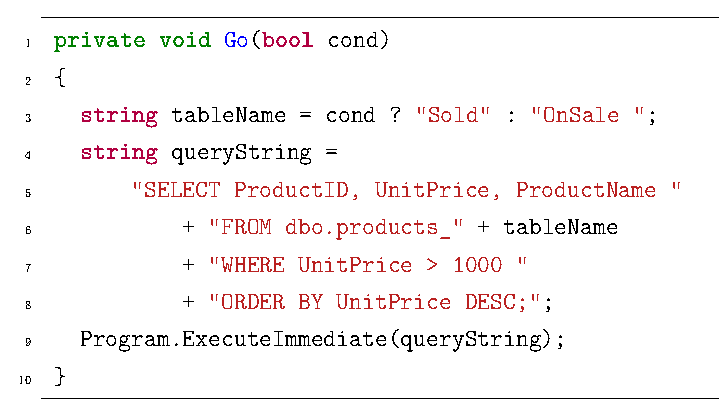
\includegraphics[width=\textwidth]{Baygeldin/pictures/intro_code.pdf}
\caption{Пример динамически формируемого кода}
\label{code_sample_1}
\end{figure}

Однако в третьей строке примера при формировании имени таблицы был пропущен пробел, и эта ошибка будет выявлена только во время выполнения программы. Таким образом, при разработке и реинжиниринге систем, использующих динамически формируемый код, можно было бы избежать множество проблем, если бы в IDE существовала поддержка статического анализа подобного кода \cite{string_embedded}. Лексический анализ является важным шагом такого статического анализа.

Задача лексического анализа — выделение лексем во входном потоке и сохранение привязки, т.е. позиции в тексте, к исходному коду. Часто при лексическом анализе используются инструменты для генерации лексических анализаторов по спецификации языка. Лексический анализатор переводит поток символов в поток лексем и может быть представлен в виде конечного преобразователя. \textbf{Конечный преобразователь} (Finite State Transducer) — это математическая модель устройства, похожая на конечный автомат, с тем лишь дополнением, что каждому переходу сопоставляется дополнительное значение, которое выводится в выходной поток. На рис.~\ref{lexer_example} продемонстрирован пример лексического анализатора языка арифметических выражений (ради простоты, единственной операций является операция сложения), представленного в виде конечного преобразователя.

\begin{figure}[h]
\centering
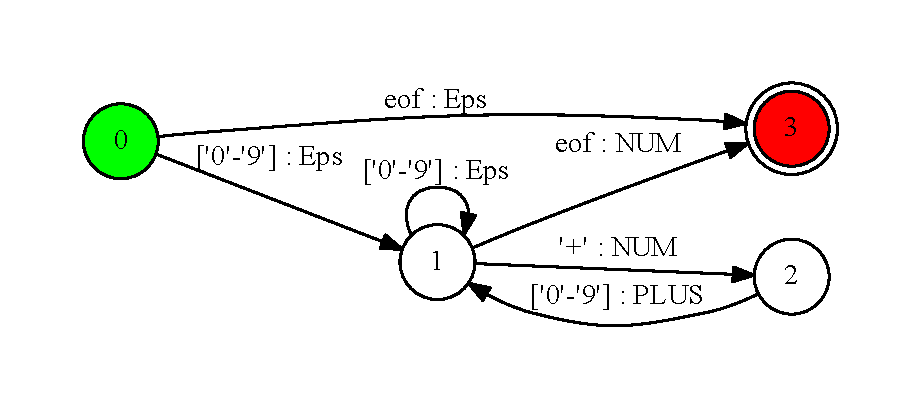
\includegraphics[width=\textwidth]{Baygeldin/pictures/lexer_.pdf}
\caption{Пример лексического анализатора, представленного в виде FST}
\label{lexer_example}
\end{figure}

Однако большинство инструментов для генерации лексических анализаторов могут работать лишь с линейным входом, что делает невозможным их непосредственное применение в нашем случае, т.к. поток символов формируется динамически. Одно из возможных решений \cite{polubelova} заключается в построении регулярной аппроксимации множества значений динамически формируемого выражения и последующем применении операции композиции \cite{handbook_automata} к двум конечным преобразователям: один их них построен по регулярной аппроксимации преобразованием автомата над строками в автомат над символами, а второй является классическим лексическим анализатором для языка, на котором написан динамически формируемый код. На рис.~\ref{reg_approx_example} изображен пример регулярной аппроксимации динамически формируемого кода, представленной в виде конечного автомата, построенного на основе кода на рис.~\ref{code_sample_2}. 

\begin{figure}[h]
\centering
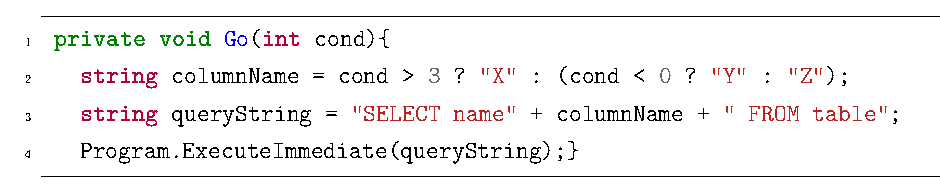
\includegraphics[width=\textwidth]{Baygeldin/pictures/approx_code.pdf}
\caption{Пример динамически формируемого кода}
\label{code_sample_2}
\end{figure}

\begin{figure}[h]
\centering
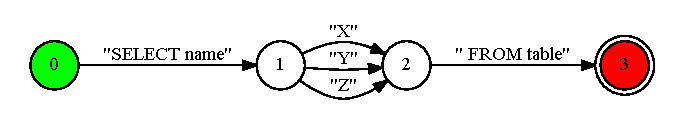
\includegraphics[width=\textwidth]{Baygeldin/pictures/approx_fsa.pdf}
\caption{Пример регулярной аппроксимации динамически формируемого кода}
\label{reg_approx_example}
\end{figure}

Результатом операции композиции конечных преобразователей является конечный преобразователь, который обладает тем свойством, что результат его работы совпадает с результатом последовательного применения участников композиции на том же входе. В нашем случае, первый конечный преобразователь переводит поток символов с их привязкой к исходному коду в поток символов, а второй (лексический анализатор) переводит поток символов в поток лексем. Таким образом, результирующий конечный преобразователь переводит поток символов с их привязкой к исходному коду в поток лексем, что и является целью лексического анализа. Результатом применения операции композиции к конечному преобразователю на рис.~\ref{operand_composition} и лексическому анализатору на рис. 2 является конечный преобразователь изображенный на рис.~\ref{composition}.

\begin{figure}[h]
\centering
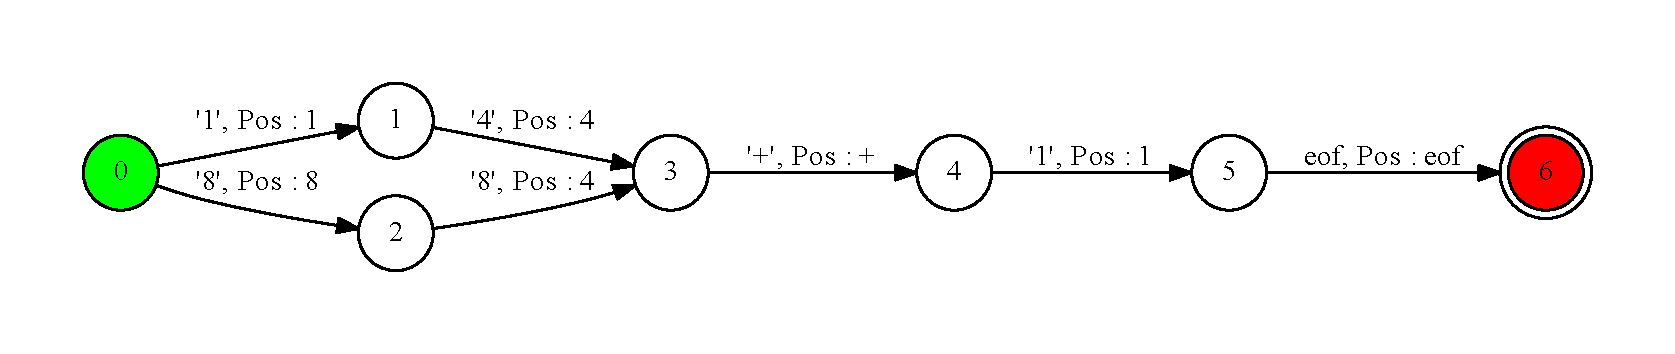
\includegraphics[width=\textwidth]{Baygeldin/pictures/example_.pdf}
\caption{Конечный преобразователь, участник операции композиции FST}
\label{operand_composition}
\end{figure}

\begin{figure}[h]
\centering
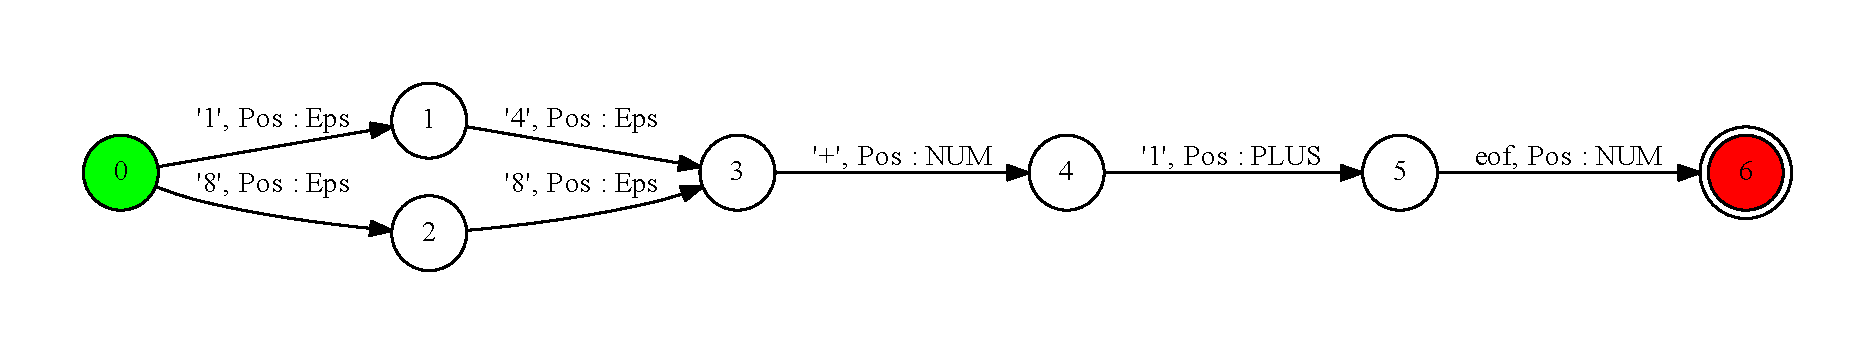
\includegraphics[width=\textwidth]{Baygeldin/pictures/res_.pdf}
\caption{Результат операции композиции FST}
\label{composition}
\end{figure}

В существующей реализации операция композиции является основной операцией в лексическом анализе динамически формируемых языков. Однако в проекте YaccConstructor \cite{yacc_article,yacc_www}, в рамках которого было реализовано такое решение \cite{polubelova}, ее производительность оказалась неудовлетворительной. Таким образом, целью данной работы являлось исследование возможности улучшения производительности лексического анализа за счет оптимизации алгоритма композиции конечных преобразователей.
